
\section{Aufbau des Projektbaums}
\label{sec:aufbau_projektbaum}
Der aus dem SVN ausgecheckte Projektbaum  ist wie folgt aufgebaut:\\
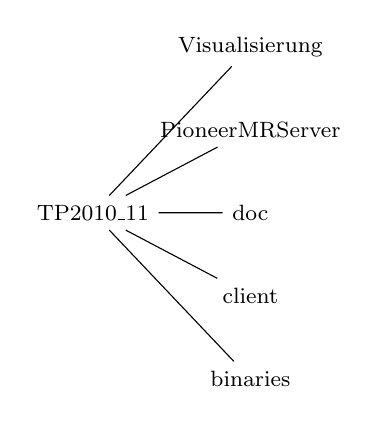
\begin{tikzpicture}
%\tikz 
[font=\footnotesize,
       grow=right, level 1/.style={sibling distance=3em},
                   level 2/.style={sibling distance=1em}, level distance=2cm]
  \node {TP2010\_11} % root
     child { node {binaries}}
     child {node {client}}
   child{node {doc} }
   child{node {PioneerMRServer}
     }
  child{node {Visualisierung}
    }; %
\end{tikzpicture}
Da beim Client es nötig war, diverse Libaries des Institutes für
Robotik und Prozessinformatik (IRP) der technischen Universität
Braunschweig sowie den Sonar-Partikelfilter und die Ballerkennung zu
integrieren, wurde dazu eine besondere Buildumgebung auf Basis von
CMake geschaffen. Sie
wird im Abschnitt \ref{cha:integr-best-proj} ab Seite
\pageref{cha:integr-best-proj} beschrieben. Einen ersten Überblick
über die Struktur des Ordners ,,client'' gibt folgende Baumübersicht:\\
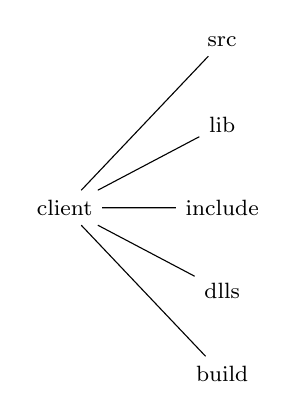
\begin{tikzpicture}
%\tikz 
[font=\footnotesize,
       grow=right, level 1/.style={sibling distance=3em},
                   level 2/.style={sibling distance=1em}, level distance=2cm]
  \node {client} % root
     child { node {build}}
     child {node {dlls}}
   child{node {include} }
   child{node {lib}
     }
  child{node {src}
    }; %
\end{tikzpicture}
Der Ordner ,,build'' enthält die durch CMake generierten VisualStudio
Projekte und fertig gebauten ausführbaren Dateien und DLLs. Die Ordner
,,dlls'' und ,,lib'' enthalten zur Erzeugung und Ausführung der
Projekte nötige externe *dll und *lib Dateien. In den Ordnern
,,include'' und ,,src'' sind schließlich die Quelltexte und Header der
verwendeten Libaries sowie unseres Clients ,,p3dxSteuerung''
enthalten. \\\\
Die Notwendigkeit einer gesondereten Buildinfrastruktur war beim
Server (PioneerMRServer) nicht 
gegeben, da dieser nicht von den Institutsbibliotheken
abhängt. Entsprecht reichte es dort, ein normales VisualStudio Projekt
zu erstellen. 

%%% Local Variables: 
%%% mode: latex
%%% TeX-master: "template"
%%% End: 
